\chapter{Methods}


\section{Design}
%-------------------------------------------%

\begin{figure}
	\caption{"Data flow within our software stack"}
	\centering
		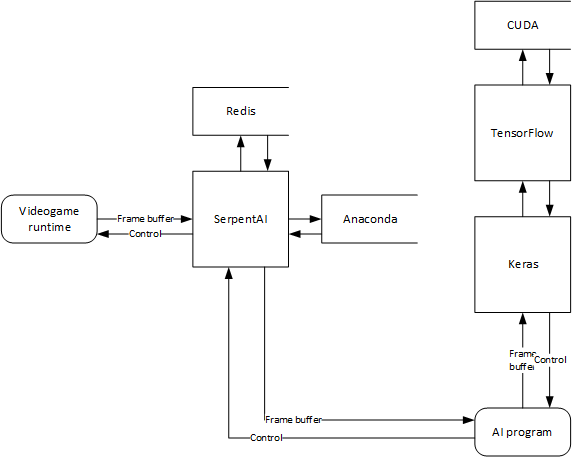
\includegraphics[scale = 0.75]{dataflow.png} \\
\end{figure}

%-------------------------------------------%


\section{Frameworks}
%-------------------------------------------%

Our project uses a software stack comprised of the following modules and libraries: {\it SerpentAI}, {\it Keras}, {\it TensorFlow}, and the {\it Anaconda Distribution} for Python 3.

We chose to use Python 3 as our primary programming language for its flexibility, intuitive syntax, and data processing capabilities. Python is also helpfully compatible with all of the other software listed above. Furthermore, the {\it Anaconda distribution} provides us with a large assortment of Python modules, some of which {\it SerpentAI} cites as dependencies \cite{SerpentAI}. This allows us to more easily work from within a Windows environment, which in turn gives us the most straightforward and stable access to GPU computation via NVIDIA proprietary drivers.

We have opted to use our own personal computers running 64-bit Windows 10 with Ubuntu subsystems as both our platform and development environment. There are several reasons to justify this decision. Firstly, we wanted to ensure that we would have the best possible experience when dealing with GPU computation, and NVIDIA simply has a longer and better track record for supporting Windows than it does for Linux. Secondly, we wanted to avoid the potential pitfall of our platform restricting us to a smaller library of target games. Our two top candidates were {\it Quake} and {\it Rivals of Aether} because both of these games support replays, or demos; however, of those two games, only {\it Quake} natively supports Linux, and ultimately we selected {\it Rivals of Aether}. Lastly, and with regards to using our own computers for both development and testing, we made the decision to abstain from distributed or cloud computing chiefly to save costs, but also as an aesthetic choice based in the desire to see what our computers are capable of. Despite all of the above justifications for using Windows, it remains to be said that our project cannot live without Linux. {\it SerpentAI} requires a Redis database, so in order for that to work we use an Ubuntu subsystem; this is the official recommendation from the {\it SerpentAI} developers \cite{SerpentAI}.

%-------------------------------------------%



\section{Algorithms}
%-------------------------------------------%


Our approach to creating this A.I. is to use a modular neural network. This neural network will use a combination of a scene segmentation algrothim to parse visual data. In addition to this we will be using a reccurrent neural-network to process inputs. The goal behind this is to have the A.I. plan its actions and learn from its guesses. 

%-------------------------------------------%



\section{Features}
%-------------------------------------------%

A brief overview of primary features you plan to implement.

%-------------------------------------------%



\section{Test Plan}
%-------------------------------------------%

We have over 1,000 data points in the form of replay files. This dataset will be randomly distributed such that around eighty-percent goes into a training set, fifteen-percent into a testing set, and the remainder into a validation set.

A training session will run as follows. The {\it SerpentAI} agent will traverse the game's menus to initiate playback of the next replay from a shuffled copy of the training set. While the match is simulated, the agent will simultaneously read the visual buffer from the game and control input data from the replay file. For each frame, the agent will pair the input data with its corresponding visual buffer and then send this bundle to a {\it TensorFlow} neural network as labels and data, respectively. The neural network will attempt to produce a set of appropriate control inputs in response and adjust its weights  whenever its prediction are incorrect. When playback has concluded, the agent will traverse the menus once again to start a new replay, repeatedly, until it has reached its quota. The total number of training iterations will vary between experiments until it produces satisfactory results.

A properly trained neural network shall demonstrate several qualities other than a high accuracy when tested against the held back data. Firstly, it shall be able to defeat low-level in-game bots, thereby demonstrating its competence. This can be tested by placing the neural network in matches against bots of increasing difficulty, thereby enabling the assignment of numerical performance benchmarks. Secondly, it shall play in a believably-human manner. This means that it should, wherever possible, be discouraged from playing {\it inhumanly} well, getting stuck, or displaying mechanical tics. Examples of these undesirable behaviors would include, in order, executing nonstop frame-perfect moves throughout the course of an entire game, running off of the stage or standing still due to an as-of-yet unseen situation, or constantly changing direction for no reason while otherwise playing competently. Identifying all such behaviors will be difficult prior to live experiments, however.

%-------------------------------------------%



\section{Criteria and Constraints}
%-------------------------------------------%

Project development must meet desired needs within realistic constraints. Many times, constraints are interrelated. Cover the appropriate criteria and constraints related to your capstone. Some example criteria and constraints are health and safety, environmental, political, social, manufacturability, sustainability, economical, and ethical.

%-------------------------------------------%
